\section{Preparation endpoints, phases, and the real commutator}
\label{sec:densityendpoints}
We retain the state, free-matter algebra, projected Gaussian operators,
proper group, units, and strict-$G_N\to0$ assumptions of
Section~\ref{sec:movingcurve}. We change only the normalized external
excess density. The limit remains $M\to\infty$ at
$t_M=\log(2M)+T$, followed by large positive or negative $T$.
The endpoint Fourier expansion is standard (DLMF 2.3.4~\cite{DLMF}); the issue here
is which complex coefficient survives taking the real part of this
particular correlator. No priority claim is made.

\subsection{Gamma densities and a two-term corner expansion}
For a fixed integer $p\ge0$ and $\beta>0$, take
\begin{equation}
 \pi_p(r)=\frac{\beta^{p+1}}{p!}r^pe^{-\beta r}\one_{r\ge0}.
 \label{eq:dep-density}
\end{equation}
Write $J_p$ for \eqref{eq:prep-moving-domain} with this density.
The square-minus-triangle formula \eqref{eq:prep-triangle} still holds.
Let $J_{p,\rm sm}$ denote the reference obtained by replacing $L_+^2$
by $L^2$ inside the $r$ integral. Its exact difference is
\begin{equation}
 J_p(\chi)-J_{p,\rm sm}(\chi)
 =\one_{\chi<0}\int_0^{-\chi}\pi_p(r)(r+\chi)^2 B(r,\chi)\dd r.
 \label{eq:dep-difference}
\end{equation}
This reference is an algebraic device, not a different projection.
Define real constants
\begin{align}
 F_\nu&=f_0(0)=\left|\Gamma(1/4+i\nu/2)\right|^4,\notag\\
 q_\nu&=\operatorname{Re}\psi(1/4+i\nu/2),&
 H_\nu&=2q_\nu+\gamma_E+2\log2,\notag\\
 d_p&=\frac{\pi p-\beta(p+1)}{p+4},&
 S_p&=\frac{\beta^{p+1}F_\nu^2}{512\pi^7}.
 \label{eq:dep-coefficients}
\end{align}
Here $H_\nu$ is a scalar coefficient, distinct from the external-leg
function $H_\nu(x,y,z)$ of Section~\ref{sec:logtime}.

\begin{lemma}[Differentiated endpoint expansion]
For $h\downarrow0$,
\begin{equation}
 J_p(-h)-J_{p,\rm sm}(-h)
 =\frac{\beta^{p+1}F_\nu^2}{(p+3)!}h^{p+3}
       \left[1+h(d_p-2iq_\nu)+O(h^2)\right].
 \label{eq:dep-corner-two}
\end{equation}
The bracket is smooth in $h$ near zero, so the remainder has its
corresponding one-sided derivative bounds.
\end{lemma}
\begin{proof}
Set $r=h\rho$, $\chi=-h$, $0\le\rho\le1$. In the unit triangle
$s,t\ge0$, $s+t<1$, its two arguments become
\[
 u=h\left(\frac12-\rho+(\rho-1)s\right),\qquad
 v=h\left(\frac12-\rho+(\rho-1)t\right).
\]
At the origin the derivatives are
\begin{equation}
 \partial_w\log f_\chi(w)\big|_{0,0}=-\pi,\qquad
 \partial_\chi\log f_\chi(w)\big|_{0,0}=iq_\nu.
 \label{eq:dep-derivatives}
\end{equation}
The Gamma factors are even in $w$ at zero, while their four digammas
sum to $4q_\nu$. The Gaussian has no first derivative there.
The triangle has area $1/2$ and mean $s+t=2/3$, hence
\[
 B(h\rho,-h)=\frac{F_\nu^2}{2}
 \left[1+h\left(-2iq_\nu-\frac\pi3+\frac{4\pi}3\rho\right)
       +O(h^2)\right].
\]
Combining this with $e^{-\beta h\rho}$, use
\[
 \int_0^1\rho^p(1-\rho)^2\dd\rho
 =\frac{2p!}{(p+3)!},\qquad
 \frac{\int_0^1\rho^{p+1}(1-\rho)^2\dd\rho}
      {\int_0^1\rho^p(1-\rho)^2\dd\rho}=\frac{p+1}{p+4}.
\]
This gives \eqref{eq:dep-corner-two}. The rescaled integration domain
is compact and all Gamma arguments stay away from poles in a common
neighborhood of $h=0$. Differentiation under the integral proves the
claimed remainder control.
\end{proof}

\subsection{Taking the real part changes the leading power}
Let $\mathcal P_p(T)=X_{\infty,p}^Q$ for $T<0$ and zero for $T>0$;
this notation specifies the two asymptotic plateaux, not an additional
time-domain term in the experiment.
\begin{theorem}[Gamma-packet ordered-time tails]
For fixed $p\in\mathbb Z_{\ge0}$ and $\beta,\nu,\sigma>0$,
\begin{equation}
 \mathcal X_p(T)-\mathcal P_p(T)
 =S_p\left[\frac{-i}{(p+3)(iT)^{p+3}}
      +\frac{-H_\nu-id_p}{(iT)^{p+4}}\right]
      +O(|T|^{-p-5}),\qquad T\to\pm\infty.
 \label{eq:dep-complex-tail}
\end{equation}
Consequently, for $s\to+\infty$,
\begin{align}
 \mathcal D_p(-s)-\mathcal D_{{\rm edge},p}
 &=\frac{2(-1)^k S_p}{p+3}s^{-p-3}+O(s^{-p-4}),
       &&p=2k,\notag\\
 &=2(-1)^{k+1}S_p d_p\,s^{-p-4}+O(s^{-p-5}),
       &&p=2k+1.
 \label{eq:dep-real-tail}
\end{align}
If $p$ is odd and $\beta=\pi p/(p+1)$, the displayed real coefficient
vanishes; this theorem then supplies an $O(s^{-p-5})$ bound, not a
nonzero leading coefficient at that order.
\label{thm:dep-gamma}
\end{theorem}
\begin{proof}
The prefactor multiplying $J_p$ in the Fourier amplitude is
\begin{equation}
 P_\sigma(\chi)=\frac{2^{2i\chi}}{512\pi^7}
   \Gamma(-i\chi)\cosh(\pi\chi/2)e^{-\sigma^2\chi^2/2}.
 \label{eq:dep-prefactor}
\end{equation}
At $\chi=-h$ it equals
\[
 P_\sigma(-h)=\frac1{512\pi^7}
       \left[-\frac ih-\gamma_E-2\log2+O(h)\right].
\]
Thus the two nonsmooth amplitude terms, expressed in $h=-\chi>0$,
are
\begin{equation}
 \frac{S_p}{(p+3)!}\left[-ih^{p+2}
                   +(-H_\nu-id_p)h^{p+3}\right]\one_{h>0}.
 \label{eq:dep-amplitude}
\end{equation}
For a smooth cutoff equal to one at $h=0$, the endpoint transform of
$h^n$ under $e^{-iTh}$ has leading term $n!/(iT)^{n+1}$.
This follows by repeated integration by parts on the half-line, with
the same formula for either sign of real $T$. It is not an absolutely
convergent transform of an uncut polynomial.

For completeness, the needed global bounds follow from Euler's Gamma
integral and its logarithmic moments. All fixed real derivatives of
$f_\chi$ are bounded by a Gaussian in $w$ times a polynomial in $w$.
The square and rescaled-triangle terms and their derivatives have at
most polynomial growth in $r,\chi$; every $r$ moment of \eqref{eq:dep-density}
is finite. Multiplication by the outer Gaussian makes all one-sided
amplitude derivatives integrable at infinity. Subtracting the PV pole
$iX_{\infty,p}^Q e^{-\chi^2}/(2\pi\chi)$ removes the remaining zero
singularity. A local smooth cutoff separates
\eqref{eq:dep-amplitude} from a smooth rapidly decreasing part. The
differentiated Taylor remainder and one further integration by parts
give $O(|T|^{-p-5})$. The subtracted pole supplies the two plateaux,
up to Gaussian-small terms. This proves \eqref{eq:dep-complex-tail}.
Finally use
$\mathcal D_p=2(N_{\infty,p}^Q-\operatorname{Re}\mathcal X_p)$ and
$\mathcal D_{{\rm edge},p}=2(N_{\infty,p}^Q-X_{\infty,p}^Q)$.
The first coefficient in \eqref{eq:dep-complex-tail} is real for even
$p$ and purely imaginary for odd $p$, giving \eqref{eq:dep-real-tail}.
\end{proof}
For $p=0$ the leading term recovers Theorem~\ref{thm:prep-moving}.
The first two complex coefficients are independent of $\sigma$ at
fixed $\sigma>0$, because its Gaussian begins contributing at second
order at this corner. Remainders and useful time ranges are not uniform
as $\sigma$ varies.

For $\beta=1$, $p=1$ has a purely imaginary $T^{-4}$ term but a
real $T^{-5}$ correction. Since $d_1=(\pi-2)/5>0$, its early
$\mathcal D_1-\mathcal D_{{\rm edge},1}$ is negative. The $p=2$
early correction is also negative. Therefore
$\mathcal D_{\rm edge}$ is an early plateau, not a universal lower
bound on $\mathcal D(T)$. This is compatible with positivity of the
full commutator norm: its plateau is strictly positive. It also
precludes universal monotone growth from the early plateau across
these preparations.

\subsection{A support gap moves the singularity away from the PV pole}
Now take a fixed gap $g>0$ and
\begin{equation}
 \pi_g(r)=\beta e^{-\beta(r-g)}\one_{r\ge g}.
 \label{eq:dep-gap-density}
\end{equation}
The projection is still $Q_M$, not $Q_{M+g}$. Only the external state
has changed. The triangle correction begins at $\chi=-g$. Writing
$\chi=-g-h$, $r=g+h\rho$ gives
\[
 J_g(-g-h)-J_{g,\rm sm}(-g-h)
 =\frac{\beta f_{-g}(-g/2)^2}{6}h^3+O(h^4).
\]
This again has differentiated one-sided remainders. Now $P_\sigma$
is regular and nonzero at $-g$, so no zero-frequency pole lowers
the corner order.
\begin{proposition}[Gapped exponential packet]
Define the nonzero complex number
\begin{equation}
 C_g=\beta P_\sigma(-g)f_{-g}(-g/2)^2.
 \label{eq:dep-gap-coefficient}
\end{equation}
With the analogous early/late plateau notation,
\begin{align}
 \mathcal X_g(T)-\mathcal P_g(T)
   &=\frac{C_g e^{-igT}}{T^4}+O(|T|^{-5}),&&T\to\pm\infty,\notag\\
 \mathcal D_g(-s)-\mathcal D_{{\rm edge},g}
   &=-\frac{2\operatorname{Re}(C_g e^{igs})}{s^4}+O(s^{-5}),
      &&s\to+\infty.
 \label{eq:dep-gap-tail}
\end{align}
The constants are for fixed $g>0$; the expansion is not uniform as
$g\downarrow0$.
\label{prop:dep-gap}
\end{proposition}
\begin{proof}
Apply the same cutoff and derivative argument at $\chi=-g$.
The transform of $h^3$ supplies $6/(iT)^4=6/T^4$, and translation
supplies $e^{-igT}$. The smooth part at $\chi=0$ retains its PV pole
and therefore the usual plateaux. All external moments remain finite.
Gamma has no zeros and no pole at the arguments in
\eqref{eq:dep-gap-coefficient}, so $C_g\ne0$.
\end{proof}
The signed early correction thus has oscillatory sign changes along
sequences of arbitrarily early ordered-limit times. Removing density
near $r=0$ has not restored the fixed-threshold exponential: it has
displaced the nonsmooth endpoint. Taking $g\to0$ before the time
asymptotic requires a separate crossover analysis.

\subsection{Direct integral checks}
For \eqref{eq:dep-density}, the survival weight is
$e^{-\beta q}\sum_{j=0}^p(\beta q)^j/j!$ for $q\ge0$
(DLMF 8.4.8). The gapped exponential uses
$e^{-\beta(q-g)_+}$. In both cases $q$ is the actual max in
\eqref{eq:mq-weight}. The first implementation integrates polynomial
moments over exact slice domains; the second uses the survival
function directly on the symmetric half-plane. No endpoint coefficient
is used in generating the full curves.

The archived runs vary transverse/Fourier orders as $(24,40)$,
$(32,40)$, and $(24,64)$ for $p=1,2$ at $\beta=1$ and for
$g=\beta=1$. They keep $\nu=0.6$, $\sigma=1$, complex amplitudes,
and separate small real differences. Local corner integrals separately
test the two-term Taylor coefficient. Numerical diagnostics and their
precision limits are reported with the data; they do not independently
certify these proof drafts, priority, or a total quadrature error.

For the numerical parameters, $H_\nu\simeq-1.65594788424$ and the
early real coefficients multiplying $s^{-5}$ are approximately
$-1.62815710723\times10^{-4}$ for $p=1$ and
$-1.42621547371\times10^{-4}$ for $p=2$. The directly integrated
real corrections divided by these signed leading terms are
\begin{center}
\begin{tabular}{rcc}
\toprule
$s=|T|$ & $p=1$ & $p=2$\\
\midrule
16 & 0.65345 & 0.62126\\
32 & 0.78681 & 0.77729\\
64 & 0.8824 & 0.8800\\
\bottomrule
\end{tabular}
\end{center}
At $T=-64$, the actual corrections are about
$-1.3380\times10^{-13}$ and $-1.1689\times10^{-13}$, respectively.
The largest observed relative changes of the small real component over
the detailed times with $|T|\le64$ are $4.64\times10^{-4}$ and
$6.62\times10^{-4}$. At $|T|=128$, the signals are only a few
$10^{-15}$ and their observed changes rise to about $0.65\%$ and
$0.95\%$. Those samples are retained but excluded from the primary
quantitative table. The visible difference from unity is a finite-time
effect, much larger than the displayed empirical refinement differences.

For $g=1$, $C_g\simeq0.000479119472+0.000588336141\,i$.
The normalized signed oscillation in Figure~\ref{fig:dep-curves}
has maximum observed refinement change about $1.74\times10^{-5}$
over its 513 plotted times. Its remaining phase and amplitude corrections
are not removed by fitting. The survival weights in all three examples
are between zero and one, so the separate real-frequency and transverse
envelope bounds of Section~\ref{sec:movingcurve} continue to apply.
They still do not certify the total PV quadrature error. The archive
contains 384 diagnostics, full complex spectra, local-corner data, and
the reduced-precision far-time samples.
\begin{figure}[htbp]
 \centering
 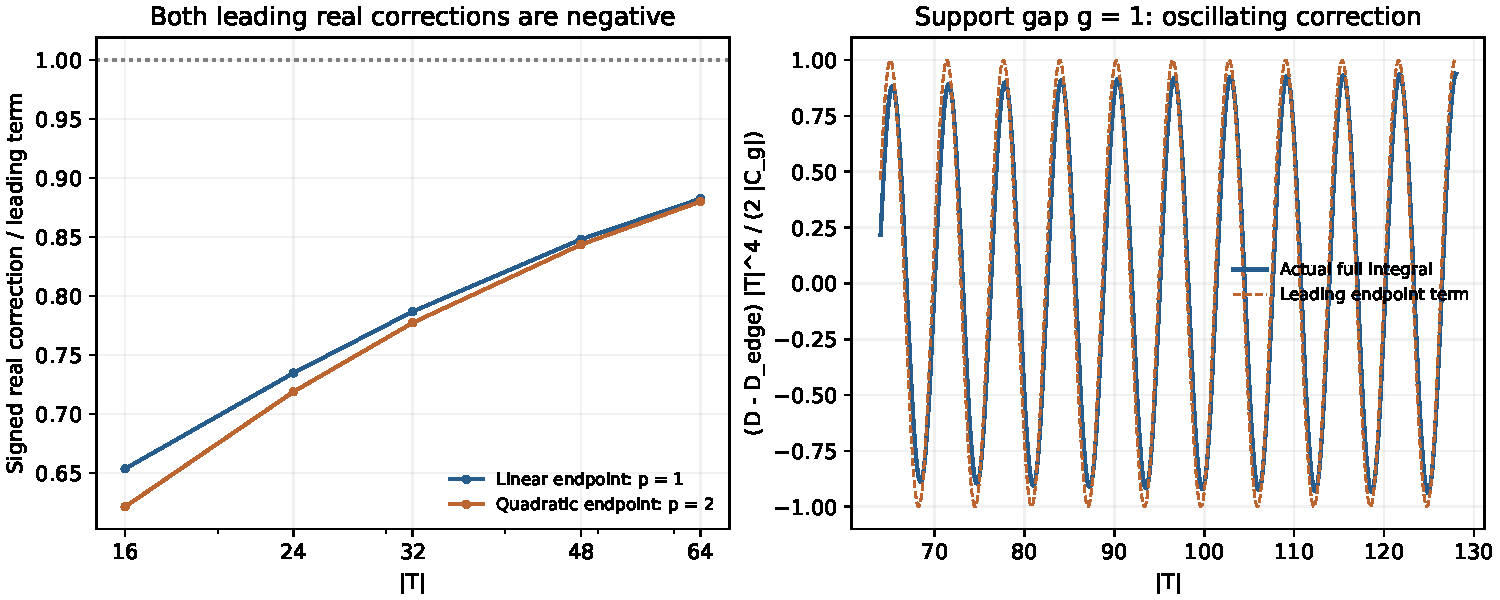
\includegraphics[width=.98\linewidth]{../results/stage3/density-endpoints/endpoint-curves.pdf}
 \caption{Actual full integrals versus endpoint predictions for
 $\nu=0.6$, $\sigma=\beta=1$. Left: ratios to the negative early
 $s^{-5}$ corrections for Gamma packets. Right: the signed early
 correction for a fixed support gap $g=1$, rescaled by $s^4/(2|C_g|)$,
 compared with $-\cos(\arg C_g+gs)$. These are empirical ordered-limit
 calculations, not finite-$M$ data.}
 \label{fig:dep-curves}
\end{figure}
